\documentclass[tikz,border=20pt]{standalone}
\usepackage{tikz}
\usetikzlibrary{shapes,arrows,positioning,fit,backgrounds,shadows}

\begin{document}
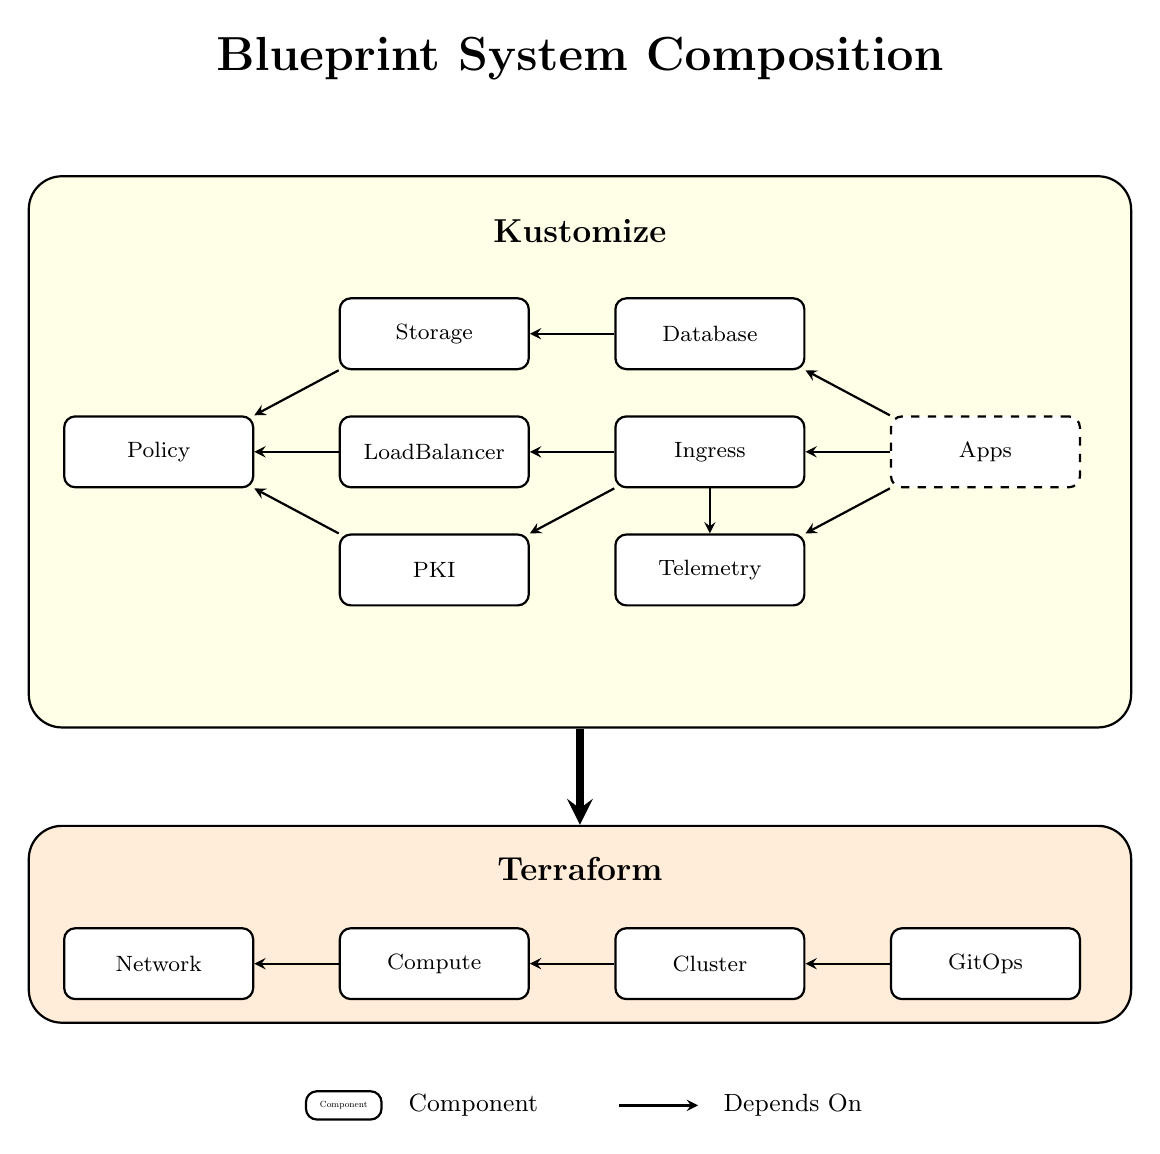
\begin{tikzpicture}[
    node distance=3.5cm and 3.5cm,
    >=stealth,
    blueprint/.style={rectangle, rounded corners=8pt, draw=black, fill=blue!15, thick, minimum width=4.5cm, minimum height=1.3cm, font=\normalsize\bfseries, drop shadow},
    terraform/.style={rectangle, rounded corners=6pt, draw=black, fill=orange!20!white, thick, minimum width=4cm, minimum height=1.1cm, font=\small\bfseries},
    kustomize/.style={rectangle, rounded corners=6pt, draw=black, fill=yellow!15!white, thick, minimum width=4cm, minimum height=1.1cm, font=\small\bfseries},
    component/.style={rectangle, rounded corners=4pt, draw=black, fill=white, thick, minimum width=2.4cm, minimum height=0.9cm, font=\footnotesize},
    arrow/.style={->, thick, color=black},
    title/.style={font=\LARGE\bfseries, color=black}
]

% Diagram title
\node[title] at (0, 11.5) {Blueprint System Composition};

% Kustomize container - contains Kubernetes-deployed components
\begin{scope}[on background layer]
    \node[rectangle, rounded corners=12pt, draw=black, fill=yellow!10!white, thick, minimum width=14cm, minimum height=7.0cm] (kustomize-bg) at (0, 6.5) {};
    \node[font=\large\bfseries, color=black] at (0, 9.3) {Kustomize};
\end{scope}

% Terraform container - contains infrastructure provisioning components
\begin{scope}[on background layer]
    \node[rectangle, rounded corners=12pt, draw=black, fill=orange!15!white, thick, minimum width=14cm, minimum height=2.5cm] (terraform-bg) at (0, 0.5) {};
    \node[font=\large\bfseries, color=black] at (0, 1.2) {Terraform};
\end{scope}

% Flow arrow showing Kustomize builds on Terraform foundation
\draw[-stealth, line width=3pt, color=black] (kustomize-bg.south) -- (terraform-bg.north);

% Kustomize layer components - Kubernetes workloads and platform services
% Left column: Security foundation
\node[component] (policy) at (-5.35, 6.5) {Policy};

% Center-left column: Core infrastructure services
\node[component] (storage) at (-1.85, 8.0) {Storage};
\node[component] (loadbalancer) at (-1.85, 6.5) {LoadBalancer};
\node[component] (pki) at (-1.85, 5.0) {PKI};

% Center-right column: Application platform services
\node[component] (database) at (1.65, 8.0) {Database};
\node[component] (ingress) at (1.65, 6.5) {Ingress};
\node[component] (telemetry) at (1.65, 5.0) {Telemetry};

% Right column: Application layer (dashed border indicates user workloads)
\node[component, dashed] (apps) at (5.15, 6.5) {Apps};

% Terraform layer components - Cloud infrastructure foundation
\node[component] (network) at (-5.35, 0.0) {Network};
\node[component] (compute) at (-1.85, 0.0) {Compute};
\node[component] (cluster) at (1.65, 0.0) {Cluster};
\node[component] (gitops) at (5.15, 0.0) {GitOps};

% Terraform dependency chain - infrastructure build order
\draw[arrow] (compute.west) -- (network.east);
\draw[arrow] (cluster.west) -- (compute.east);
\draw[arrow] (gitops.west) -- (cluster.east);

% Kustomize dependency graph - service dependencies within Kubernetes
% Policy enforcement dependencies (diagonal connections to corners)
\draw[arrow] (storage.south west) -- (policy.north east);
\draw[arrow] (pki.north west) -- (policy.south east);
% Load balancer requires policy foundation
\draw[arrow] (loadbalancer.west) -- (policy.east);
% Ingress layer dependencies
\draw[arrow] (ingress.west) -- (loadbalancer.east);
\draw[arrow] (ingress.south west) -- (pki.north east);
% Application layer dependencies
\draw[arrow] (apps.west) -- (ingress.east);
\draw[arrow] (apps.north west) -- (database.south east);
\draw[arrow] (apps.south west) -- (telemetry.north east);
% Data layer connection
\draw[arrow] (database.west) -- (storage.east);
% Monitoring connection
\draw[arrow] (ingress.south) -- (telemetry.north);

% Legend - positioned below the diagram with better spacing
\begin{scope}[shift={(0,-1.8)}]
    % Component legend item
    \node[component, scale=0.4] at (-3.0,0) {Component};
    \node[right, font=\small] at (-2.3,0) {Component};

    % Arrow legend item with more space
    \draw[-stealth, thick, color=black] (0.5,0) -- (1.5,0);
    \node[right, font=\small] at (1.7,0) {Depends On};
\end{scope}


\end{tikzpicture}
\end{document}
